\chapter{State-of-the-Art}\label{chap:state-art}
\todo{write about PE data}
In the demand for an effective, high-quality approach to the analysis of isolates from infected animals, molecular studies help to investigate characteristics of the sample. Genome analysis has become an integral part of animal disease surveillance, especially since the advent of high-throughput sequencing technologies in the last 15 years. Next-generation techniques and applications are described below, the state of the art in poxvirus and avian influenza virus detection and analysis, and lastly the drawbacks of the methods are discussed.

\section{High-throughput Technologies in Diagnostic Virology}

When comparing DNA sequencing technologies, there are differences in speed, throughput and volume of sequences. The term ''next generation'' used to describe newer technologies in the field implies a next step in the evolution of sequencing technologies. As sequencing machine technologies evolve rapidly, there are gradations such as ''second generation'' and ''third generation''. Following the original 1977 Sanger sequencing method using radioactivity and gels, second generation sequencers are advancements of Sanger sequencing using sequencing by synthesis~\cite{mardis2008next}. The reactions run in parallel and drastically reduce overall costs. Third-generation sequencing technologies typically generate longer primary reads of DNA (and RNA) molecules while maintaining the parallelism of the technology and taking advantage of this benefit~\cite{slatko2018overview}. The most commonly used next-generation technologies for DNA sequencing and their applications are described below.

\subsection{Overview of NGS Platforms and Applications}
By far the biggest player in the field of DNA sequencing today is the Illumina platform, first developed by Solexa and Lync Therapeutics. Illumina sequencing is based on bridge amplification, which creates clusters of copies of each DNA fragment. This technique involves repeated synthesis reactions with proprietary modified nucleotides containing a different fluorescent label for each of the four bases A, T, C and G. The reactions are performed over 300 or more rounds, and fluorescent detection allows for faster detection through direct imaging. An Illumina sequencer outputs data in the form of sequence reads, which are short DNA fragments ranging from 50 to 600 base pairs in length, depending on the specific instrument and protocol used~\cite{illumina2015introduction, slatko2018overview, mardis2008next}. The output data from an Illumina sequencer is typically in the form of raw sequence files in FASTQ format, which contain the base calls and corresponding quality scores for each read. These reads can be used for downstream analyses such as viral genome assembly and variant calling.

Oxford Nanopore Technologies (ONT) is one of the third generation sequencing technologies and is a paradigm shifting platform. It measures changes in ionic current accross membranes as single-stranded DNA nucleotides pass through a nanopore~\cite{jain2016oxford}. Nanopore-based DNA sequencing technologies like ONT come as a portable, small MinION device, allowing experts to use it for many applications where space requirements or portability are important~\cite{greninger2015rapid, jain2016oxford}. Despite its advantages, the main caveat of ONT is its relatively high error rate compared to other HTS methods~\cite{fu2019comparative}. This makes ONT less suitable for single-nucleotide variant analysis that is required in some diagnostic applications~\cite{bowden2019sequencing, stefan2022comparison}.

Other frequently used platforms are Roche/454 sequencing, Ion Torrent technology and SOLiD (Sequencing by Oligonucleotide Ligation and Detection). Fourth-generation platforms include single molecule real-time sequencing (SMRT) by PacBio and nanopore sequencing~\cite{rhoads2015pacbio}. 

\begin{figure}
	\centering
	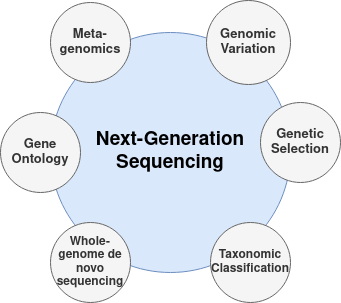
\includegraphics[width=0.5\textwidth]{media/other/ngs.png}
	\caption{Overview of next-generation sequencing technology applications in diagnostic virology.}
	\label{fig:ngs}
\end{figure}

As NGS platforms are widely used in biomedical contexts, some of the most important applications in diagnostic virology are depicted in Figure~\ref{fig:ngs}. In virology, metagenomics can be used to identify viruses in complex clinical samples~\cite{chiu2019clinical}. This technique allows for the detection of known and novel viruses without prior knowledge of the infectious agent. Metagenomics involves the sequencing of all genetic material in a sample, including viral genomes, to identify the presence of viruses. If a virus is identified, genomic variation refers to differences in the DNA sequence of a virus between different strains or isolates. These variations can be used to track the spread of an outbreak, identify the source of an infection, or determine the level of virulence of a virus~\cite{capobianchi2013next}. \\
Genetic selection refers to the process by which certain viral strains become more prevalent in a population over time due to selective pressures. In diagnostic virology, genetic selection can be used to track the evolution of a virus over time and determine which strains are most likely to cause outbreaks or epidemics. This is of special interest in the backtracing of infected animals to know where the virus came from. \\
Using gene ontology, functions and interactions of genes are described. This is crucial in order to identify the genes responsible for specific viral functions and to understand how these functions contribute to viral pathogenesis. \\
Based on their genetic and structural characteristics, viruses are classified to existing systems, called taxonomic classification. This clustering analysis can be used to identify the type of virus causing an infection and determine its potential for transmission and pathogenicity~\cite{dutilh2021perspective}.\\
Whole-genome de novo sequencing refers to the sequencing of an entire viral genome without prior knowledge of its genetic sequence. Similar to metagenomics, this technique can be used to identify novel viruses and to track the evolution of a virus over time~\cite{slatko2018overview}.

\subsection{Detection of Viral Pathogens}
- NGS-based methods: VIDISCA protocol for SARS-CoV in 2004
- metagenomics-based strategies: higher sensitivity (compared to microarray-based assays), detect full spectrum of viruses
- NGS-based: Illumina GA platform for detection of new viruses (influenza A) and de novo assembly (only works with high enough number of reads generated)
- bats: coronavirus consensus PCR and unbiased HTS (high-throughput pyrosequencing) -> reveal presence of sequences of new coronavirus related to SARS-CoV

\subsection{Data Analysis Issues}

no standardization of techniques \\
no knowledge sharing/best practices/common source of knowledge \\
livestock diseases do not receive much attention from bioinformaticians and therefore not enough monitoring;
although in regions where outbreaks have larger impacts on economy and other fields, the surveillance is crucial for prevention and control.

This emphasizes the importance of free and easy-access platforms like Galaxy that entitle professionals to analyse their samples. Technical know-how to develop and maintain servers for analysis of NGS data is not a global standard and also not needed everywhere when multidisciplinary approaches can be shared through platforms.

costs are relatively high, especially for countries or health organizations in development countries that are still affected by diseases they want to monitor

%%%%%%%%%%%

Illumina shows low coverage of AT rich regions~\cite{harismendy2009evaluation}

* chimerical sequences (artifacts originating from joining sequences), point mutations, insertions/deletions which occur during reverse transcription, PCR amplification or sequencing itself
* cleaning step or filtering phase removes low-quality reads from the dataset, while the error correction separates true variants from those due to experimental noise. -> idea that errors are randomly distributed with low frequency, and real mutations are clustered and their abundance are quantified

Each application of software with NGS data requires expertise in resolving limitations and drawbacks of specific methods. This in turn requires bioinformatic skills and the careful interpretation of results. Still, NGS provides a large pool of methods which eases the tasks, although available algorithms for genome assembly and amplicon analysis have drawbacks and limitations~\cite{finotello2012comparative}.

% WOAH/FAO: Network of Expertise on Animal Influenza
% WHO: GISRS (Global Influenza Surveillance and Response System) for human influenza,
% WHO: FluNet
% WHO: GISAID (Global Initiative on Sharing All Influenza Data)
% \cite{daniels2023health}

\section{NGS Methods for Poxviruses}

difference/similarities between monkeypox, goat pox, sheep pox etc. \\
advances in surveillance (4 genera of poxviruses are zoonotic and may infect humans)

classification based on phenotypic characteristics.

\subsection{Poxviruses}
viral disease that affects cattle, transmission through blood-feeding insects such as ticks or some species of mosquitoes and flies. \\
* symptoms \\
vaccination programme (mass-vaccination by EU commission protecting >1.8million cattle)\\
spreading in African countries, since 2012 present in middle east to south-east europe

Zoonotic poxviruses

Transmission modes, limited host range 

2 subfamilies, one infects vertebrates and one infects insects
-> 10 genera infect vertebrates

characteristic ITR that is left out in other pipelines (Yale University primer scheme starts after and ends before ITR)

with monkeypox outbreak in 2022, professionals of the field had the event to examine another pox virus, seeing similarities among pox viruses motivates to extend existing pipelines for data analyses to work with samples of all pox viruses

one poxvirus to mention in more detail:
Lumpy Skin Disease (LSD) is caused by the virus belonging to the Capripoxvirus (CaPV) genus within the family Poxviridae, subfamily Chordopoxvirinae~\cite{walker2019changes}. The LSDV genome is a double-stranded linear DNA molecule of circa 151 kilobasepairs in length. It contains between 147 and 156 open reading frames. With a sequence identity of over 96\% with the other CaPV genus members sheep pox and goatpox, the lSDV genome is very similar to the other CaPV genomes~\cite{tulman2001genome}. These three viruses of the capripoxvirus genus are the most serious poxvirus diseases of livestock in terms of economic losses in the case of an outbreak. 

One strain of LSDV that has been extensively studied is the Neethling strain, first isolated in Kenya in 1958. It constitutes the strain used for the live-attenuated vaccine that is widely used for cattle against LSDV outbreaks. Similar to other poxviruses, the LSDV genome consists of a central coding region which is bounded by two identical inverted terminal repeat (ITR) regions with a length of circa 2,400 basepairs at both ends of the genome. This is a key characteristic to consider during reconstruction of the genome. 

capripox not transmissable to humans -> NOT a zoonosis

\subsection{Application of NGS Technologies in Poxvirus Diagnostics}

https://www.sciencedirect.com/science/article/pii/S0166093422000118 explains Primer scheme and why tiling amplicon approach makes sense even for large genome size of CaPV genome and complex structure with repetitive ITR regions


\section{NGS Methods for Avian Influenza Virus}\label{sec:AIV}
\subsection{Avian Influenza Virus}

informally known as bird flu, the avian influenza is a viral infectious disease whose hosts are wild waterbirds. \\
occurring in two variants determining the severeness, therefor low/highly pathogenic and in a variety of subtypes, that are composed by two viral segments H1-H16 in combination with N1-N11 \\

* symptoms

* LPAIV, HPAIV

* Etiology: virus composition, taxonomy, origin, mutation rates

Human Influenza Virus:
AIV has more subtypes as there are more prevalent subtypes in many different populations; more variants

\subsection{Application of NGS Technologies in Avian Influenza Virus Diagnostics}
surveillance systems include classical phylogenetic methods to genotype novel emerging strains, classify viral lineages or assess tree topologies to distinguish between novel and emerging strains (taxonomic classification -- there are many strains)
%%%%%
SARS-CoV-2 tracking is of huge global interest, resulting in a highly regarded topic with ongoing scientific activity in terms of publications \\
includes established institutions in bioinformatics that hand out approaches, guidelines, recommendations to govern outbreaks of viral livestock diseases. includes comprehensive pipelines for bioinformaticians, veterinarians and other health professionals.
major platforms that offer exhaustive approaches to analyse genomic samples from infected stock. \\

INSaFLU, ViReflow? (SARS-CoV-2 samples) \\
 VAPOR (ref datasets) \\

* INSaFLU (inside the flu) -> for influenza, NGS towards metagenomic virus detection, routine genomic surveillance, 

* Nextstrain -> for RT SARS-CoV-2, Influenza, Ebola pathogen populations 
* Kraken2 -> taxonomic sequence classifier (using database and k-mers of FASTA sequences)
* VirFind (by Arkansas High Performance Computing Center) -> for fasta/Illumina fastq files, to detect new samples (trimming, mapping to ref, de novo assembly, Blastn, Blastx)
* ARTIC Network -> RAMPART for Ebola, yellow fever virus (read assignment, mapping, phylogenetic analysis on ONT data)
* IRIDA -> Integrated Rapid Infectious Disease Analysis for NGS data e.g. de novo assembly (FLAsh, SPAdes, Prokka)


tracking viruses using genomic sequence data collection; effective surveillance does not require exhaustive case surveillance, instead the collection of enough data from representative populations. This enables health professionals to detect newly evolved variants and to monitor trends in the circulating variants.\\
wastewater

https://synapse.koreamed.org/articles/1134050